
\documentclass[border=10pt, 12pt]{standalone}
\usepackage[svgnames]{xcolor}
\usepackage{amsmath}
\usepackage{pgfplots}
\pgfplotsset{compat=newest}
\usepackage[sfdefault]{FiraSans}
\usepackage{FiraMono}
\renewcommand*\familydefault{\sfdefault}
\begin{document}
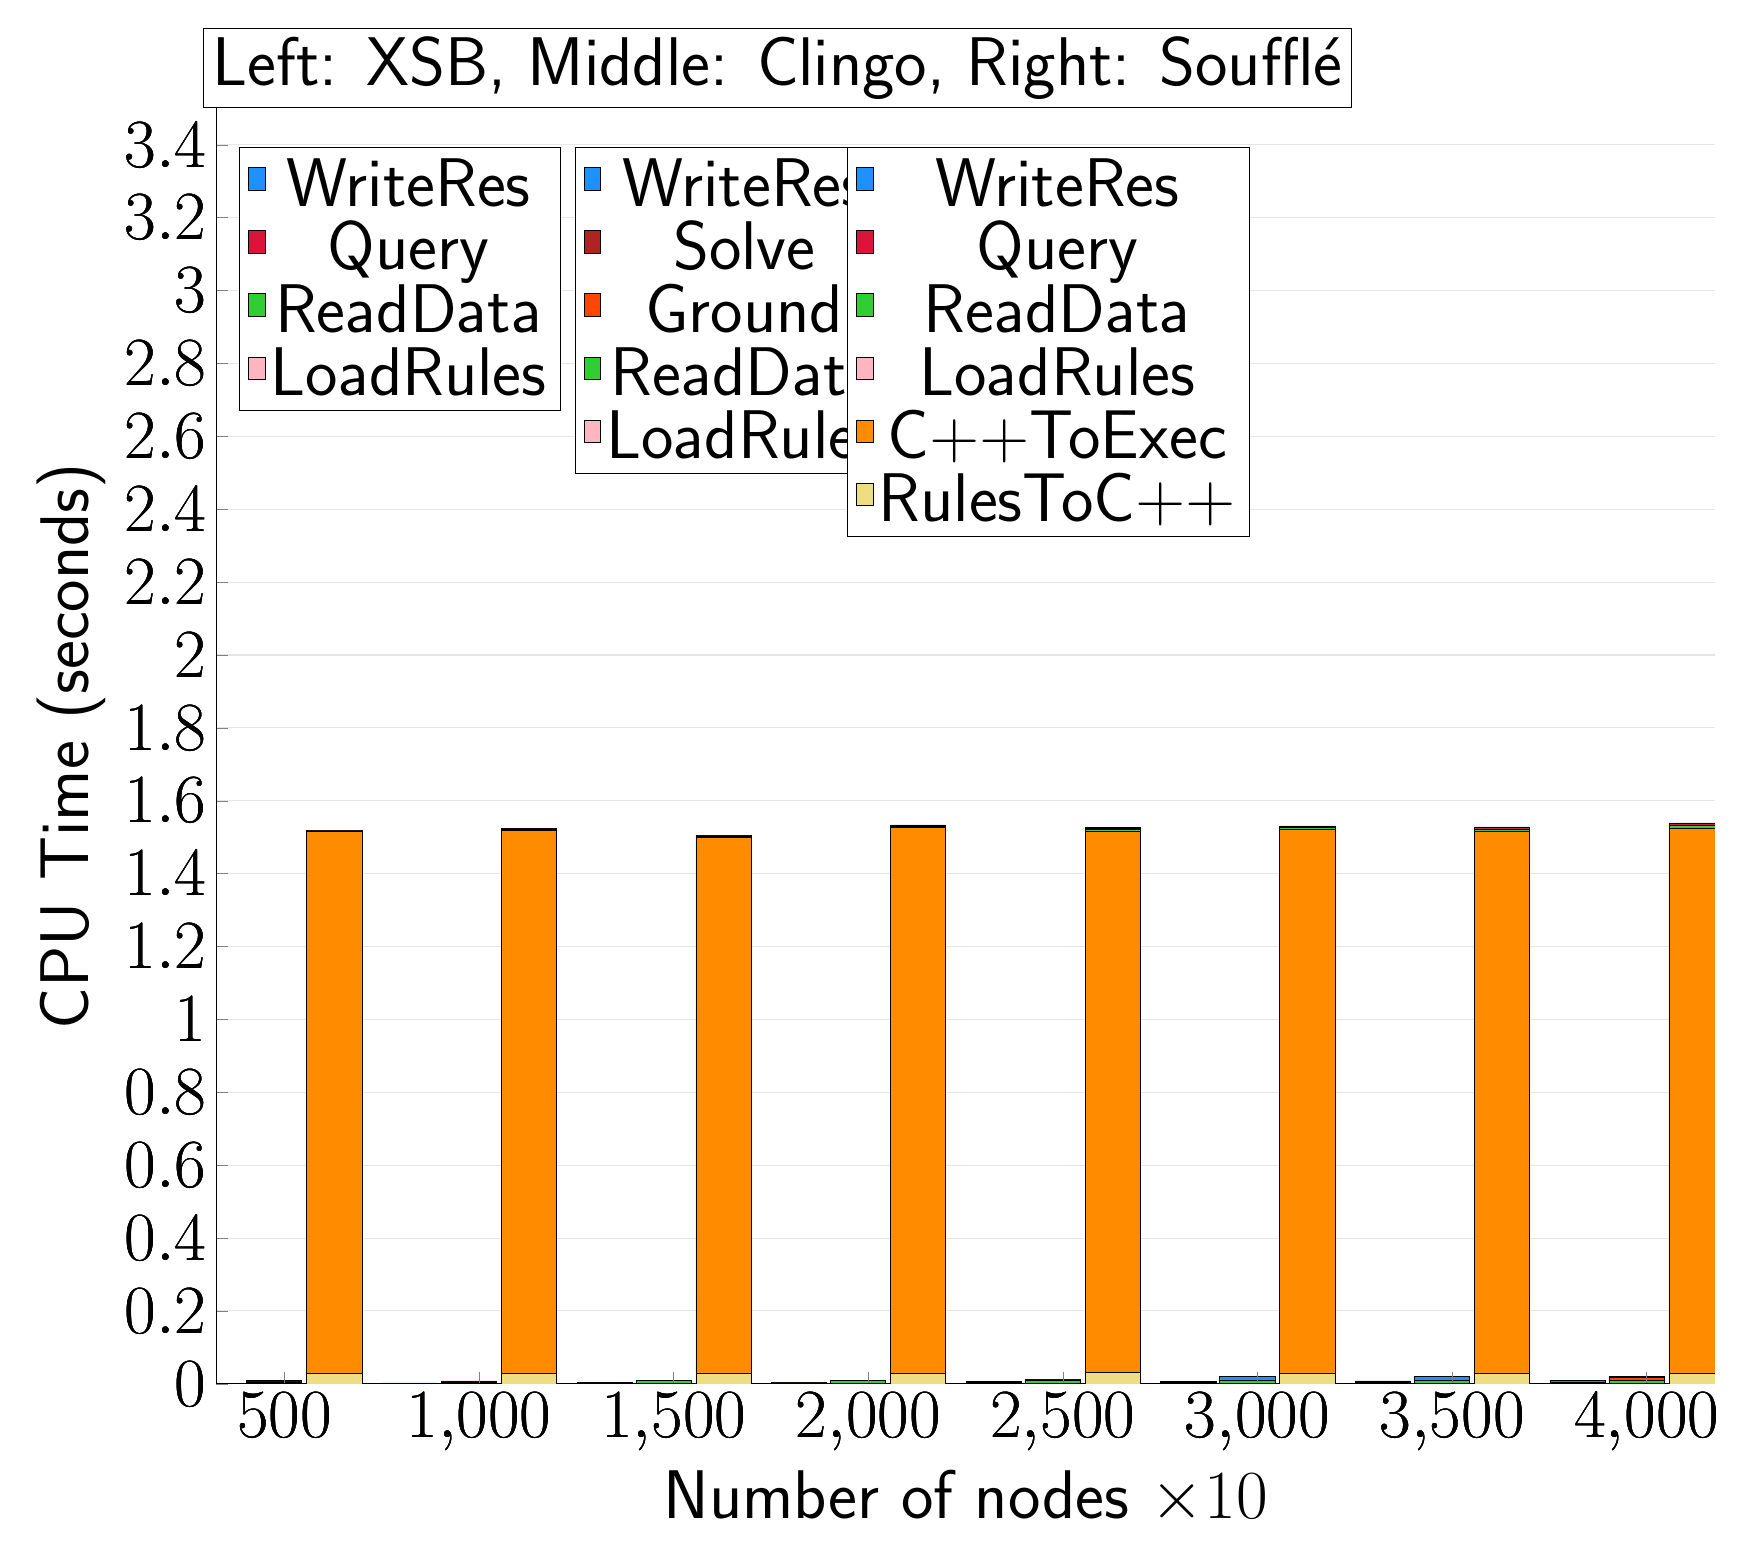
\begin{tikzpicture}
	\begin{axis}[bar shift=-25pt,
			ybar stacked,
			width=1.7\textwidth,
			bar width=0.7cm,
			ymajorgrids, tick align=inside,
			major grid style={draw=gray!20},
			xtick=data,
			ymin=0, ymax=3.5,
			axis x line*=bottom,
			axis y line*=left,
			enlarge x limits=0.05,
			legend style={
					at={(0.23, 0.97)},
					anchor=north east,
					legend columns=1,
					font=\Huge,
				},
			ylabel={CPU Time (seconds)},
			xlabel={Number of nodes $\times 10$},
			label style={font=\Huge},
			tick label style={font=\Huge},
		]
		\addlegendimage{fill=DodgerBlue, draw=black, line width=0.2pt}
		\addlegendentry{WriteRes}
		\addlegendimage{fill=Crimson, draw=black, line width=0.2pt}
		\addlegendentry{Query}
		\addlegendimage{fill=LimeGreen, draw=black, line width=0.2pt}
		\addlegendentry{ReadData}
		\addlegendimage{fill=LightPink, draw=black, line width=0.2pt}
		\addlegendentry{LoadRules}
		\addplot +[fill=LightPink, draw=black, line width=0.2pt] coordinates {
				(500, 0.0005996)
				(1000, 0.0006213000000000002)
				(1500, 0.0006450000000000001)
				(2000, 0.0006138999999999998)
				(2500, 0.0006094)
				(3000, 0.0006635999999999998)
				(3500, 0.0006411999999999998)
				(4000, 0.0006245000000000003)
			};
		\addplot +[fill=LimeGreen, draw=black, line width=0.2pt] coordinates {
				(500, 0.0005417999999999996)
				(1000, 0.0009953000000000004)
				(1500, 0.0015178999999999998)
				(2000, 0.0019105)
				(2500, 0.0023179000000000003)
				(3000, 0.0028798)
				(3500, 0.0032356999999999998)
				(4000, 0.0036857999999999995)
			};
		\addplot +[fill=Crimson, draw=black, line width=0.2pt] coordinates {
				(500, 8.940000000000041e-05)
				(1000, 0.0001718999999999993)
				(1500, 0.0002629000000000002)
				(2000, 0.0003371000000000002)
				(2500, 0.0004903000000000002)
				(3000, 0.0006750000000000003)
				(3500, 0.0008247)
				(4000, 0.0009096)
			};
		\addplot +[fill=DodgerBlue, draw=black, line width=0.2pt] coordinates {
				(500, 0.0005165999999999997)
				(1000, 0.0009742000000000006)
				(1500, 0.0014110999999999996)
				(2000, 0.0018723999999999998)
				(2500, 0.0023401)
				(3000, 0.0030097999999999995)
				(3500, 0.0033907)
				(4000, 0.003825)
			};
	\end{axis}

	\begin{axis}[bar shift=-3.7pt,
			ybar stacked,
			width=1.7\textwidth,
			bar width=0.7cm,
			ymajorgrids, tick align=inside,
			major grid style={draw=none},
			xtick=data,
			ymin=0, ymax=3.5,
			axis x line*=none,
			axis y line*=none,
			enlarge x limits=0.05,
			legend style={
					at={(0.454, 0.97)},
					anchor=north east,
					legend columns=1,
					font=\Huge,
				},
			label style={font=\Huge},
			tick label style={font=\Huge},
		]
		\addlegendimage{fill=DodgerBlue, draw=black, line width=0.2pt}
		\addlegendentry{WriteRes}
		\addlegendimage{fill=FireBrick, draw=black, line width=0.2pt}
		\addlegendentry{Solve}
		\addlegendimage{fill=OrangeRed, draw=black, line width=0.2pt}
		\addlegendentry{Ground}
		\addlegendimage{fill=LimeGreen, draw=black, line width=0.2pt}
		\addlegendentry{ReadData}
		\addlegendimage{fill=LightPink, draw=black, line width=0.2pt}
		\addlegendentry{LoadRules}
		\addplot +[fill=LightPink, draw=black, line width=0.2pt] coordinates {
				(500, 0.0)
				(1000, 0.0)
				(1500, 0.0019999999999999996)
				(2000, 0.0)
				(2500, 0.0)
				(3000, 0.0)
				(3500, 0.0)
				(4000, 0.0)
			};
		\addplot +[fill=LimeGreen, draw=black, line width=0.2pt] coordinates {
				(500, 0.004999999999999999)
				(1000, 0.004999999999999999)
				(1500, 0.007999999999999997)
				(2000, 0.009999999999999997)
				(2500, 0.010999999999999998)
				(3000, 0.009999999999999997)
				(3500, 0.009999999999999997)
				(4000, 0.009999999999999997)
			};
		\addplot +[fill=OrangeRed, draw=black, line width=0.2pt] coordinates {
				(500, 0.0019999999999999996)
				(1000, 0.0029999999999999996)
				(1500, 0.0)
				(2000, 0.0)
				(2500, 0.0)
				(3000, 0.0)
				(3500, 0.0)
				(4000, 0.007000000000000001)
			};
		\addplot +[fill=FireBrick, draw=black, line width=0.2pt] coordinates {
				(500, 0.0)
				(1000, 0.0)
				(1500, 0.0)
				(2000, 0.0)
				(2500, 0.0)
				(3000, 0.0)
				(3500, 0.0)
				(4000, 0.0010000000000000002)
			};
		\addplot +[fill=DodgerBlue, draw=black, line width=0.2pt] coordinates {
				(500, 0.0029999999999999996)
				(1000, 0.0)
				(1500, 0.0)
				(2000, 0.0)
				(2500, 0.0010000000000000002)
				(3000, 0.010000000000000004)
				(3500, 0.010000000000000004)
				(4000, 0.0030000000000000005)
			};
	\end{axis}

	\begin{axis}[bar shift=18pt,
			ybar stacked,
			width=1.7\textwidth,
			bar width=0.7cm,
			ymajorgrids, tick align=inside,
			major grid style={draw=none},
			xtick=data,
			ymin=0, ymax=3.5,
			axis x line*=none,
			axis y line*=none,
			enlarge x limits=0.05,
			legend style={
					at={(0.69, 0.97)},
					anchor=north east,
					legend columns=1,
					font=\Huge,
				},
			label style={font=\Huge},
			tick label style={font=\Huge},
		]
		\addlegendimage{fill=DodgerBlue, draw=black, line width=0.2pt}
		\addlegendentry{WriteRes}
		\addlegendimage{fill=Crimson, draw=black, line width=0.2pt}
		\addlegendentry{Query}
		\addlegendimage{fill=LimeGreen, draw=black, line width=0.2pt}
		\addlegendentry{ReadData}
		\addlegendimage{fill=LightPink, draw=black, line width=0.2pt}
		\addlegendentry{LoadRules}
		\addlegendimage{fill=DarkOrange, draw=black, line width=0.2pt}
		\addlegendentry{C++ToExec}
		\addlegendimage{fill=LightGoldenrod, draw=black, line width=0.2pt}
		\addlegendentry{RulesToC++}
		\addplot +[fill=LightGoldenrod, draw=black, line width=0.2pt] coordinates {
				(500, 0.030000000000000006)
				(1000, 0.030000000000000006)
				(1500, 0.030000000000000006)
				(2000, 0.030000000000000006)
				(2500, 0.031000000000000007)
				(3000, 0.030000000000000006)
				(3500, 0.030000000000000006)
				(4000, 0.030000000000000006)
			};
		\addplot +[fill=DarkOrange, draw=black, line width=0.2pt] coordinates {
				(500, 1.486)
				(1000, 1.4890000000000003)
				(1500, 1.4699999999999998)
				(2000, 1.496)
				(2500, 1.4860000000000002)
				(3000, 1.491)
				(3500, 1.485)
				(4000, 1.4949999999999999)
			};
		\addplot +[fill=LightPink, draw=black, line width=0.2pt] coordinates {
				(500, 7.41e-05)
				(1000, 0.000101)
				(1500, 0.00011060000000000002)
				(2000, 0.0001104)
				(2500, 8.319999999999999e-05)
				(3000, 6.860000000000001e-05)
				(3500, 0.0001209)
				(4000, 0.00011)
			};
		\addplot +[fill=LimeGreen, draw=black, line width=0.2pt] coordinates {
				(500, 0.001131)
				(1000, 0.0024238)
				(1500, 0.0034053)
				(2000, 0.0044318)
				(2500, 0.0052959)
				(3000, 0.0060579)
				(3500, 0.0077147)
				(4000, 0.008284999999999999)
			};
		\addplot +[fill=Crimson, draw=black, line width=0.2pt] coordinates {
				(500, 0.0004376999999999999)
				(1000, 0.0010538)
				(1500, 0.0015428)
				(2000, 0.0019511)
				(2500, 0.0024622000000000003)
				(3000, 0.0028393000000000003)
				(3500, 0.003624)
				(4000, 0.0041826)
			};
		\addplot +[fill=DodgerBlue, draw=black, line width=0.2pt] coordinates {
				(500, 0.00037520000000000007)
				(1000, 0.0006571000000000001)
				(1500, 0.0008213)
				(2000, 0.0010425)
				(2500, 0.0011975000000000002)
				(3000, 0.001309)
				(3500, 0.0016054000000000003)
				(4000, 0.0016965)
			};
	\end{axis}


	\node[anchor=south, draw, fill=white] at (rel axis cs:0.42,1) {\Huge Left: XSB, Middle: Clingo, Right: Soufflé};
\end{tikzpicture}
\end{document}
